\section{Resultados}

O tipo de plantação base usado para esse trabalho foi a Cana-de-açúcar, mas outros tipos de plantio foram testados e se obteve o resultado desejado. Por esse motivo os resultados que serão apresentados, tem como plantio base a Cana-de-açúcar.

Segue abaixo algumas das regras de produção utilizadas: 

\begin{figure}[h!]
\centering
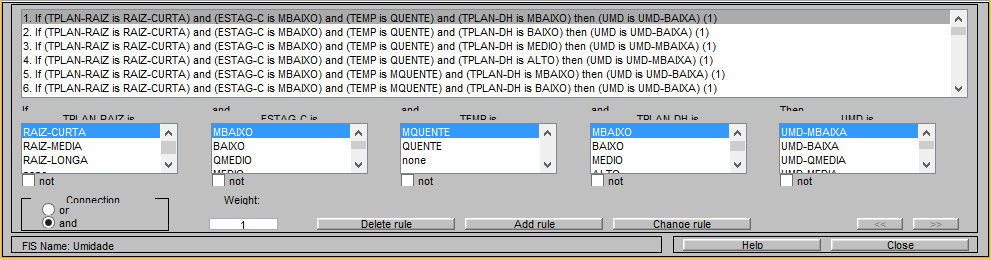
\includegraphics[width=1\linewidth]{Resultados/Imagens/regras}
\caption{Regras de produção}
\label{fig:Regras}
\end{figure}

Como exemplo começaremos atribuindo os seguintes valores para as variáveis de entrada:

\textbf{TPLAN-RAIZ:} RAIZ-MEDIA (onde há uma necessidade de água maior em relação a \textbf{RAIZ-CURTA} e menor que a \textbf{RAIZ-LONGA}).

\textbf{ESTAG-C:} BAIXO (estágio de germinação, momento onde a planta necessita de menos água durante a sua vida).

\textbf{TEMP:} QUENTE (necessita de mais água devido a temperatura).

\textbf{TPLAN-DH:} BAIXO (possui uma baixa resistência a perda de água do solo).

Obtemos o seguinte resultado:

\begin{figure}[h!]
\centering
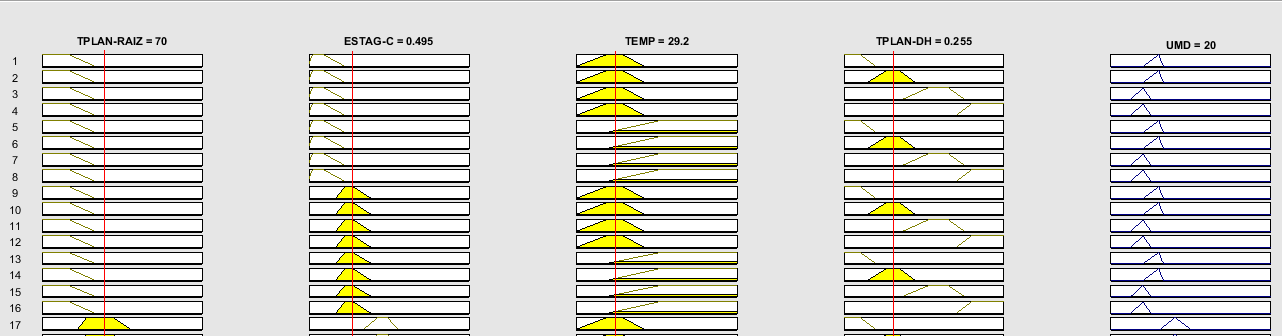
\includegraphics[width=1\linewidth]{Resultados/Imagens/resultado1}
\caption{Resultado 1}
\label{fig:resultado1}
\end{figure}

Nessas condições a variável de saída \textbf{UMD} é igual a 20 (umidade média). Se alterarmos as variáveis de entrada da seguinte forma:  

\textbf{TPLAN-RAIZ:} RAIZ-MEDIA (requer a mesma quantidade de água da configuração anterior).

\textbf{ESTAG-C:} ALTO (estágio de floração, onde a planta necessita de mais água).

\textbf{TEMP:} MQUENTE (necessita ainda mais água devido a temperatura).

\textbf{TPLAN-DH:} BAIXO (mesma valor da configuração anterior).

Obtemos o seguinte resultado:

\begin{figure}[h!]
\centering
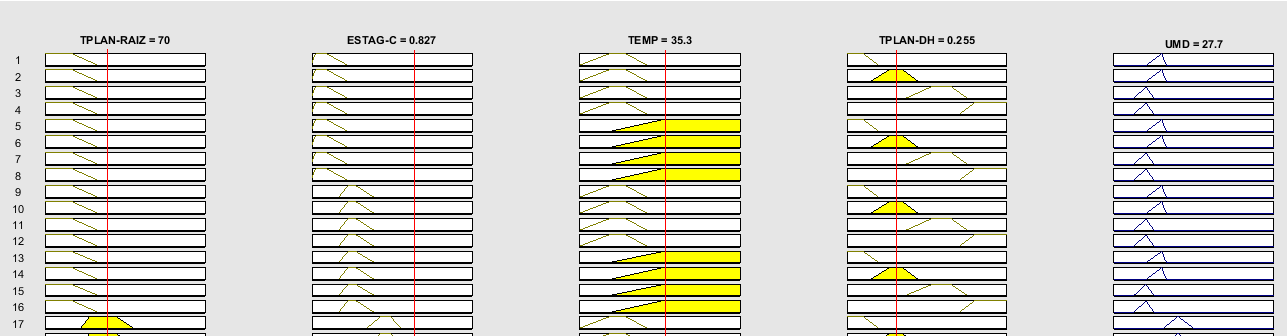
\includegraphics[width=1\linewidth]{Resultados/Imagens/resultado2}
\caption{Resultado 2}
\label{fig:resultado2}
\end{figure}

Como esperado com o estágio de crescimento da planta alterado para alto, o qual requer um maior consumo hídrico, e a temperatura alterada para muito quente, a umidade ideal para o solo aumenta para 27,7 (umidade alta). Com base nesses resultados concluímos que o sistema \fuzzy implementado correspondeu as expectativas do projeto. 

\subsection{Vídeo apresentação}

\textbf{Link:} \url{https://youtu.be/Mbm_Qy1ufrY} 
